\documentclass{standalone}

\usepackage{graphicx}

\usepackage{tikz}

\usetikzlibrary{positioning}
\usetikzlibrary{arrows.meta}
\usetikzlibrary{calc}

\begin{document}

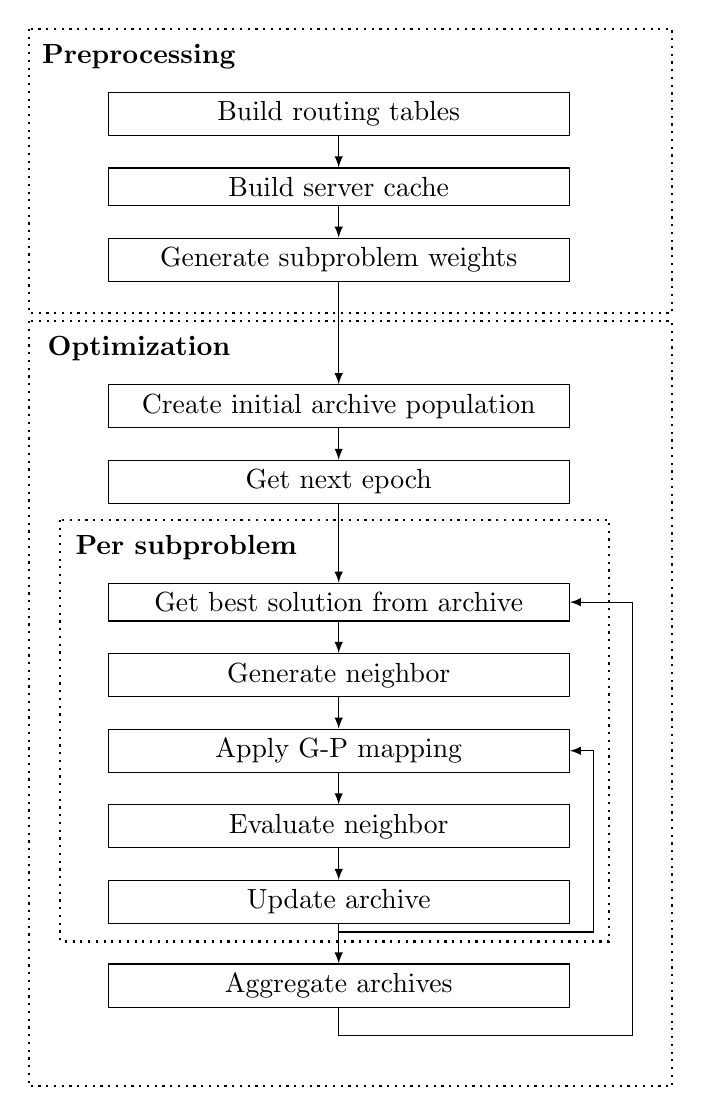
\begin{tikzpicture}[
    block/.style={align=center, rectangle, draw=black, fill=white, text width=16em},
]
    \node[block] (I1) [] {Build routing tables};
    \node[block] (I2) [below=0.4cm of I1] {Build server cache};
    \node[block] (I3) [below=0.4cm of I2] {Generate subproblem weights};

    \node[block] (B2) [below=1.3cm of I3] {Create initial archive population};
    \node[block] (B3) [below=0.4cm of B2] {Get next epoch};

    \node[block] (B4) [below=1cm of B3] {Get best solution from archive};
    \node[block] (B5) [below=0.4cm of B4] {Generate neighbor};
    \node[block] (B6) [below=0.4cm of B5] {Apply G-P mapping};
    \node[block] (B7) [below=0.4cm of B6] {Evaluate neighbor};
    \node[block] (B8) [below=0.4cm of B7] {Update archive};

    \node[block] (B9) [below=.5cm of B8] {Aggregate archives};

    \node[] (H1) [below=0.1cm of B9] {};
    \node[] (H2) [right=0.8cm of B4] {};

    \draw[-latex] (I1.south) -- (I2.north);
    \draw[-latex] (I2.south) -- (I3.north);
    \draw[-latex] (I3.south) -- (B2.north);
    \draw[-latex] (B2.south) -- (B3.north);
    \draw[-latex] (B3.south) -- (B4.north);
    \draw[-latex] (B4.south) -- (B5.north);
    \draw[-latex] (B5.south) -- (B6.north);
    \draw[-latex] (B6.south) -- (B7.north);
    \draw[-latex] (B7.south) -- (B8.north);
    \draw[-latex] (B8.south) -- (B9.north);
    % \draw[-latex] (B9.south) -- (B10.north);

    \draw[-latex] (B9.south) -| (H1.south) -| (H2.west) -- (B4.east);
    \draw[-latex] (B8.south) -| ($(B8.south)+(0,-0.1)$) -| ($(B6.east)+(0.3,0)$) -- (B6.east);
    
    \draw[thick,dotted] ($(I1.north west)+(-1,0.8)$) rectangle ($(I3.south east)+(1.3,-.4)$);
    \node[] at ($(I1.north west)+(0.4,0.45)$) {\textbf{Preprocessing}};

    \draw[thick,dotted] ($(B2.north west)+(-1,0.8)$) rectangle ($(B9.south east)+(1.3,-1)$);
    \node[] at ($(B2.north west)+(0.4,0.45)$) {\textbf{Optimization}};

    \draw[thick,dotted] ($(B4.north west)+(-0.6,0.8)$) rectangle ($(B8.south east)+(0.5,-0.22)$);
    \node[] at ($(B4.north west)+(1,0.45)$) {\textbf{Per subproblem}};

\end{tikzpicture}

\end{document}